\subsection{The indenter experiment}\label{sec:indenter}
The indenter benchmark simulate a rigid punch on a purely plastic von Mises material, for which exists an analytical solution \citep{Thieulot2008,Thieulot2014,Glerum2018}.

\begin{wrapfigure}{r}{9.5cm}
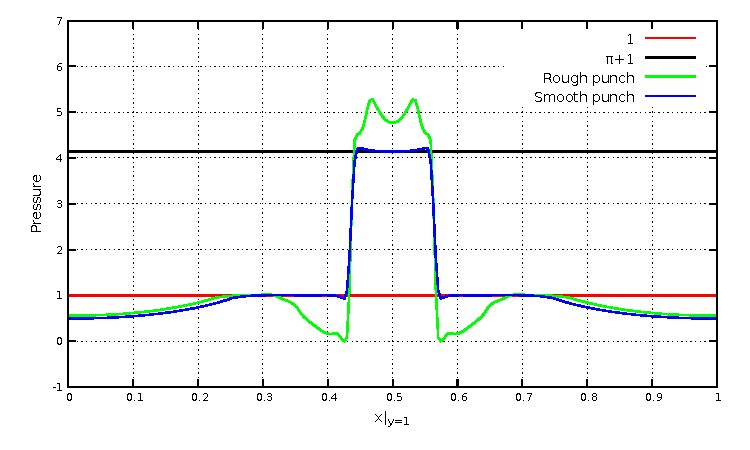
\includegraphics[width=9.5cm]{./Figures/Smooth_Rough.pdf}
\caption{Nodal pressure in function of the x coordinate at $y=1$ for rough (green line) and smooth (blue line) punch experiment. Black and red lines indicate
the analytical solution at $x=0.5$ and $x=0.5 \pm w_p$, respectively.}
\label{fig:smooth_p}
\end{wrapfigure}
The domain is a unit square with a grid resolution of $256\times256$ elements. The gravity acceleration is set to $\bm{g}=\bm{0}$ and effective viscosity is capped using $\eta_{min}=10^{-4}$ and $\eta_{max}=10^3$. The tolerance for the convergence of the non-linear solution is $tol=10^{-9}$, with a maximum number of non-linear iterations set to 500. The medium in the domain has $\rho=0.01$, an initial viscosity $\eta_0=10$, cohesion $C=1$ and an angle of internal friction $\phi=0$°. Velocity boundary conditions are set to no slip at the bottom and free slip at the sides of the domain. The top of the domain is open with the exception of the central portion (punch area) with width $w_p=0.125$, where $v=-1.05$ and $u$ is fixed either to 0 (rough punch experiment) or free (smooth punch experiment).

The analytical solution indicate that pressure at ($0.5;1$) and ($0.5 \pm w_p;1$)is $p=\pi +1$ and $p=1$, respectively
(black and red lines in Fig. \ref{fig:smooth_p}). Fig. \ref{fig:smooth_p} shows a clear improvement in the pressure solution when passing from a rough to a
smooth punch (green and blue lines in Fig. \ref{fig:smooth_p}, respectively), as previously observed by \citet{Thieulot2014} and \citet{Glerum2018}.
Fig. \ref{fig:indenter} show the results in terms of viscosity (panels a and b), strain rate (panels c and d), velocity (panels e and f) and pressure
(panels g and h) for both experiments.
All data can be found at \url{https://github.com/aleregorda/Benchmarks/tree/main/Nonlinear_visco_plasticity/Indenter}.

\begin{figure}[h!]
\centering
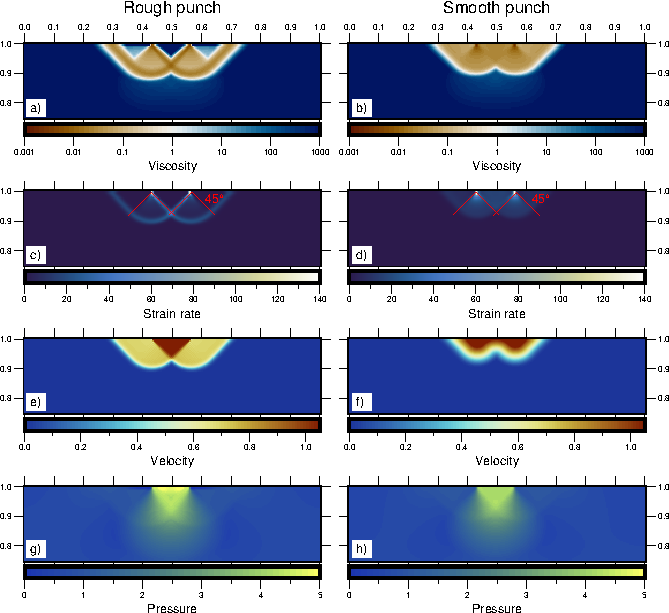
\includegraphics[width=14cm]{./Figures/Indenter.pdf}
\caption{Viscosity (panels a and b), strain rate (panels c and d), velocity (panels e and f) and pressure (panels g and h) fields for rough (left column) and
smooth (right column) punch experiments.}
\label{fig:indenter}
\end{figure}